\chapter[Future work and Proposed simulations]{Future work and Proposed 
simulations}

\section{Summary}
The need for this work has been shown by a summary of the current state of the 
art of \gls{MSR} depletion simulator capabilities. The literature review in 
Chapter 1 concluded that most \gls{MSR} depletion simulators typically assume 
ideal (rather than realistically constrained) poison removal rates for the 
nuclear system performance modeling. Moreover, most of the simulators assumed 
constant extraction efficiency vectors, which must be determined by the user 
in the input file and cannot be a function of other parameters. The Python 
toolkit, SaltProc v1.0, will directly couple with the Serpent 2 Monte Carlo 
depletion code for liquid-fueled \gls{MSR} depletion simulation to enable 
realistic online reprocessing system modeling. The SaltProc v1.0 seeks to be a 
universal tool for fuel composition evolution analysis in \glspl{MSR} with 
taking into account the complex fuel salt reprocessing system. Such 
reprocessing systems may consist of multiple components with variable removal 
efficiencies and rates. Moreover, these components can be connected in series, 
parallel, or a combination, which will be accurately treated in the SaltProc 
v1.0. Section~\ref{sec:reproc-plant} details the generic design of \gls{MSR}  
fuel salt reprocessing systems. Section~\ref{sec:tool_design} describes the  
SaltProc v1.0 architecture and design that is required to successfully model 
comprehensive liquid-fueled \glspl{MSR} with online fuel reprocessing systems. 

Figure~\ref{fig:workflow} shows an outline of this work. The current chapter 
details each Stage of the proposed work.
 \begin{sidewaysfigure}[ht!] % replace 't' with 'b' to force it to 
 	\centering
 	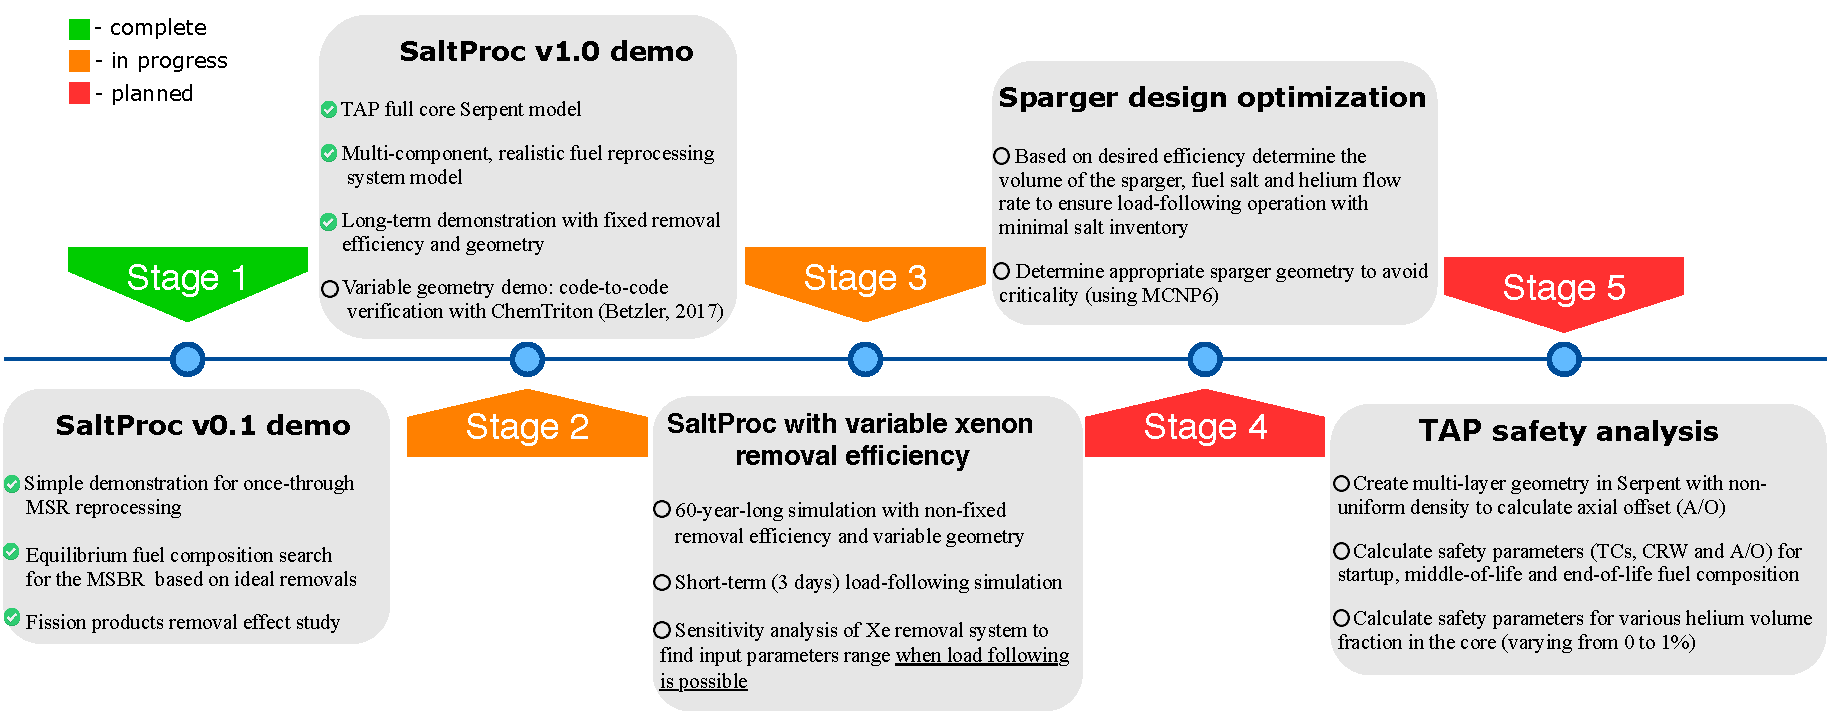
\includegraphics[width=1.06\textwidth]{progress_chart.pdf} 
 	\caption{Workflow for the simulations proposed in this work.}
 	\label{fig:workflow}
 \end{sidewaysfigure}
 \FloatBarrier
 
 
\section{Stage 1: Basic online reprocessing demonstration}
In Stage 1, \gls{MSR} online reprocessing simulation capabilities have been 
reviewed and summarized (Chapter 1). SaltProc v0.1 was demonstrated for 
simplified burnup calculation for the \gls{MSBR} as a part of my M.Sc. thesis  
\cite{rykhlevskii_advanced_2018} and published paper  
\cite{rykhlevskii_modeling_2019}. These efforts illuminated depletion of the 
fuel salt in the \gls{MSBR} for 60 years of operation and took into account 
the following processes:
\begin{enumerate}
	\item \gls{FP} removal from the salt with fixed, ideal extraction 
	efficiencies (the fuel reprocessing system removed 100\% of target 
	poisons).
	\item $^{233}$Pa removal (100\%) and feed of an equal mass of $^{233}$U 
	into the core (instantaneous $^{233}$Pa decay to $^{233}$U was assumed).
	\item Fresh fertile material ($^{232}$Th) feed to maintain the constant 
	fuel salt inventory.
\end{enumerate}
Additionally, the effect of removing fission products from the fuel salt was 
investigated separately for a different group of \glspl{FP} (noble gases, 
noble and seminoble metals, rare earth elements). As expected, removing  
fission products provides significant neutronic benefit and enables a longer 
core lifetime. Section~\ref{sec:pre-results-msbr} described key findings after 
completing Stage 1.

\section{Stage 2: SaltProc v1.0 demonstration and validation for the TAP}
Simulating a realistic multi-component fuel reprocessing system is important 
for calculating an accurate fuel salt composition. SaltProc v0.1 was 
completely refactored for modeling a complicated salt reprocessing system. To 
demonstrate SaltProc v1.0 capabilities, we have created a full-core \gls{TAP} 
\gls{MSR} model in Serpent 2 \cite{chaube_tap_2019} which was described in 
detail in Section~\ref{sec:tap_model}. Moreover, the multi-component fuel 
reprocessing system of the \gls{TAP} was developed on this stage 
(Section~\ref{sec:stage2-demo}). Section~\ref{sec:stage2-demo} also presented 
preliminary results of Stage 2. The Stage 2 demonstration case has following 
advantages over Stage 1:
\begin{itemize}
	\item SaltProc v0.1 (Stage 1) approximated the fuel salt reprocessing 
	system 
	as a single ``black'' box, which removes the entire mass (100\% removal 
	efficiency) of processed elements at once. In contrast, SaltProc v1.0 
	treats the fuel reprocessing system as a complex structure of components, 
	each removing a specific set of elements with specific extraction 
	efficiency. 
	\item SaltProc v1.0 inherently checks mass conservation at each depletion 
	step and dynamically calculates feed stream to maintain the fuel salt 
	inventory constant.
	\item SaltProc v1.0 tracks the waste stream from each component.
\end{itemize}

The foremost future effort in this stage is to enable switching between 
multiple Serpent geometries during simulation. For the \gls{TAP} concept, the 
number of moderator rods in the core varies from 1332 at the startup to 6700 
at the \gls{EOL}. The user will have an option to choose when SaltProc v1.0 
should switch to next geometry: (1) after a specific depletion  time (e.g., 18 
months which is a common maintenance/refueling shutdown interval for 
\glspl{LWR}); or (2) when the effective multiplication factor reaches a 
specific value (e.g., $1.00<k_{eff} < 1.002$). Additionally, SaltProc v1.0 
will correct the total fuel salt inventory in the primary loop to compensate 
for the core geometry change. Overall, the adjustable geometry capability will 
realistically simulate long-term (60 year) operation of the \gls{TAP} reactor 
to obtain accurate fuel salt composition at different moments during operation.

Results obtained in Stage 2 will be used for code-to-code verification with  
ChemTriton/Shift results for full-core \gls{TAP} core geometry from the most 
recent \gls{ORNL} technical report TM-2017/475 \cite{betzler_assessment_2017}. 
Notably, the fuel salt composition evolution during the \gls{TAP} reactor 
operation and corresponding core geometry are determinative for all next 
stages.

This work is developed with a test-driven development paradigm. Specifically, 
before any new functionality is implemented, a suite of tests is written, 
which as carefully define its expected behavior as possible. The code is then 
written to pass the test suite. In this way, the tool developed in this work 
is expected to be comprehensively tested in parallel with its development. 
Thus, after code-to-code verification with ChemTriton/Shift multiple-component 
integration tests will be added to the test harness to make sure that future 
changes in the code will not break previous functionality.

Test problems will help comprehensively define and confirm each unit of the 
demonstration functionality. These problems will include fundamental, 
information-passing tests as well as more challenging multiple-component 
integration tests. Every unit of functionality within the toolkit will be 
tested as an integral part of development.

This milestone will result in a processing system model capable of simulating
various liquid-fueled \glspl{MSR} with multi-component fuel reprocessing 
systems but with constant separation efficiencies, defined at runtime. 
Additionally, this stage will demonstrate a key feature of the \gls{TAP} 
\gls{MSR} - adjusting the moderator rod configuration - which is necessary to 
maintain the reactor criticality during the 60-years lifetime. 

\section{Stage 3: Variable xenon extraction rate} \label{sec:xe-removal-rate}
When Stage 2 is complete, a series of extensions to the Stage 2 model will 
be pursued. These will incorporate extraction efficiencies as a function of 
many physical system design parameters (e.g., void fraction in the salt, 
helium bubble size). Mathematical correlations for the efficiencies will be 
taken from relationships in the literature \cite{peebles_removal_1968, 
gabbard_development_1974} and CFD simulations currently being conducted 
at the University of Illinois at Urbana-Champaign \cite{huff_enabling_2018}. 
For demonstration proposes, just xenon removal efficiency will be defined as a 
function of many parameters (Section~\ref{sec:gas-separ}) due to 
limited data provided in the listed literature. For other fission products  
from the \gls{TAP} reprocessing scheme (table~\ref{tab:reprocessing_list}), 
removal efficiencies will be defined based on the removal rates from the 
table, assuming time-independent extraction efficiency. This milestone will 
result in a realistic online reprocessing system model capable of modeling 
\gls{MSR} systems with parameterized, realistically achievable process rates,  
and extraction efficiencies.

Another anticipated extension will test the \gls{TAP} reactor ability to 
operate in a load-following regime. Short-term (3 days) depletion using 
SaltProc v1.0 will be performed with the core power changing in the [0, 100\%] 
range with a ramp rate 10\%/min (to be competitive with natural gas peaking 
plants, which ramp at or above 10\% of their capacity) 
\cite{huff_enabling_2018}. 
Figure~\ref{fig:load} shows the load curve selected to demonstrate the 
worst-case scenario of load-following:
\begin{enumerate}
	\item Startup with fresh fuel and operating on 100\% of \gls{HFP}
level 
	for 40 hours to reach $^{135}$Xe/$^{135}$I equilibrium;
	\item Load-following power drop (0.1 \gls{HFP}/min), from \gls{HFP} 
	to \gls{HZP};
	\item Shutdown for 8 hours\footnote{At startup. Time after shutdown when 
	$^{135}$Xe concentration would reach maximum value greatly depends on 
	neutron energy spectrum which for the \gls{TAP} concept changes 
	significantly during operation.} to reach the $^{135}$Xe peak;
	\item Load-following power rise (0.1 \gls{HFP}/min), from \gls{HZP} 
	to \gls{HFP}.
\end{enumerate}
This scenario can be considered as backing up solar power with
nuclear on a high-solar penetration grid (e.g., in California).
\begin{figure}[bth!] % replace 't' with 'b' to 
	\centering
	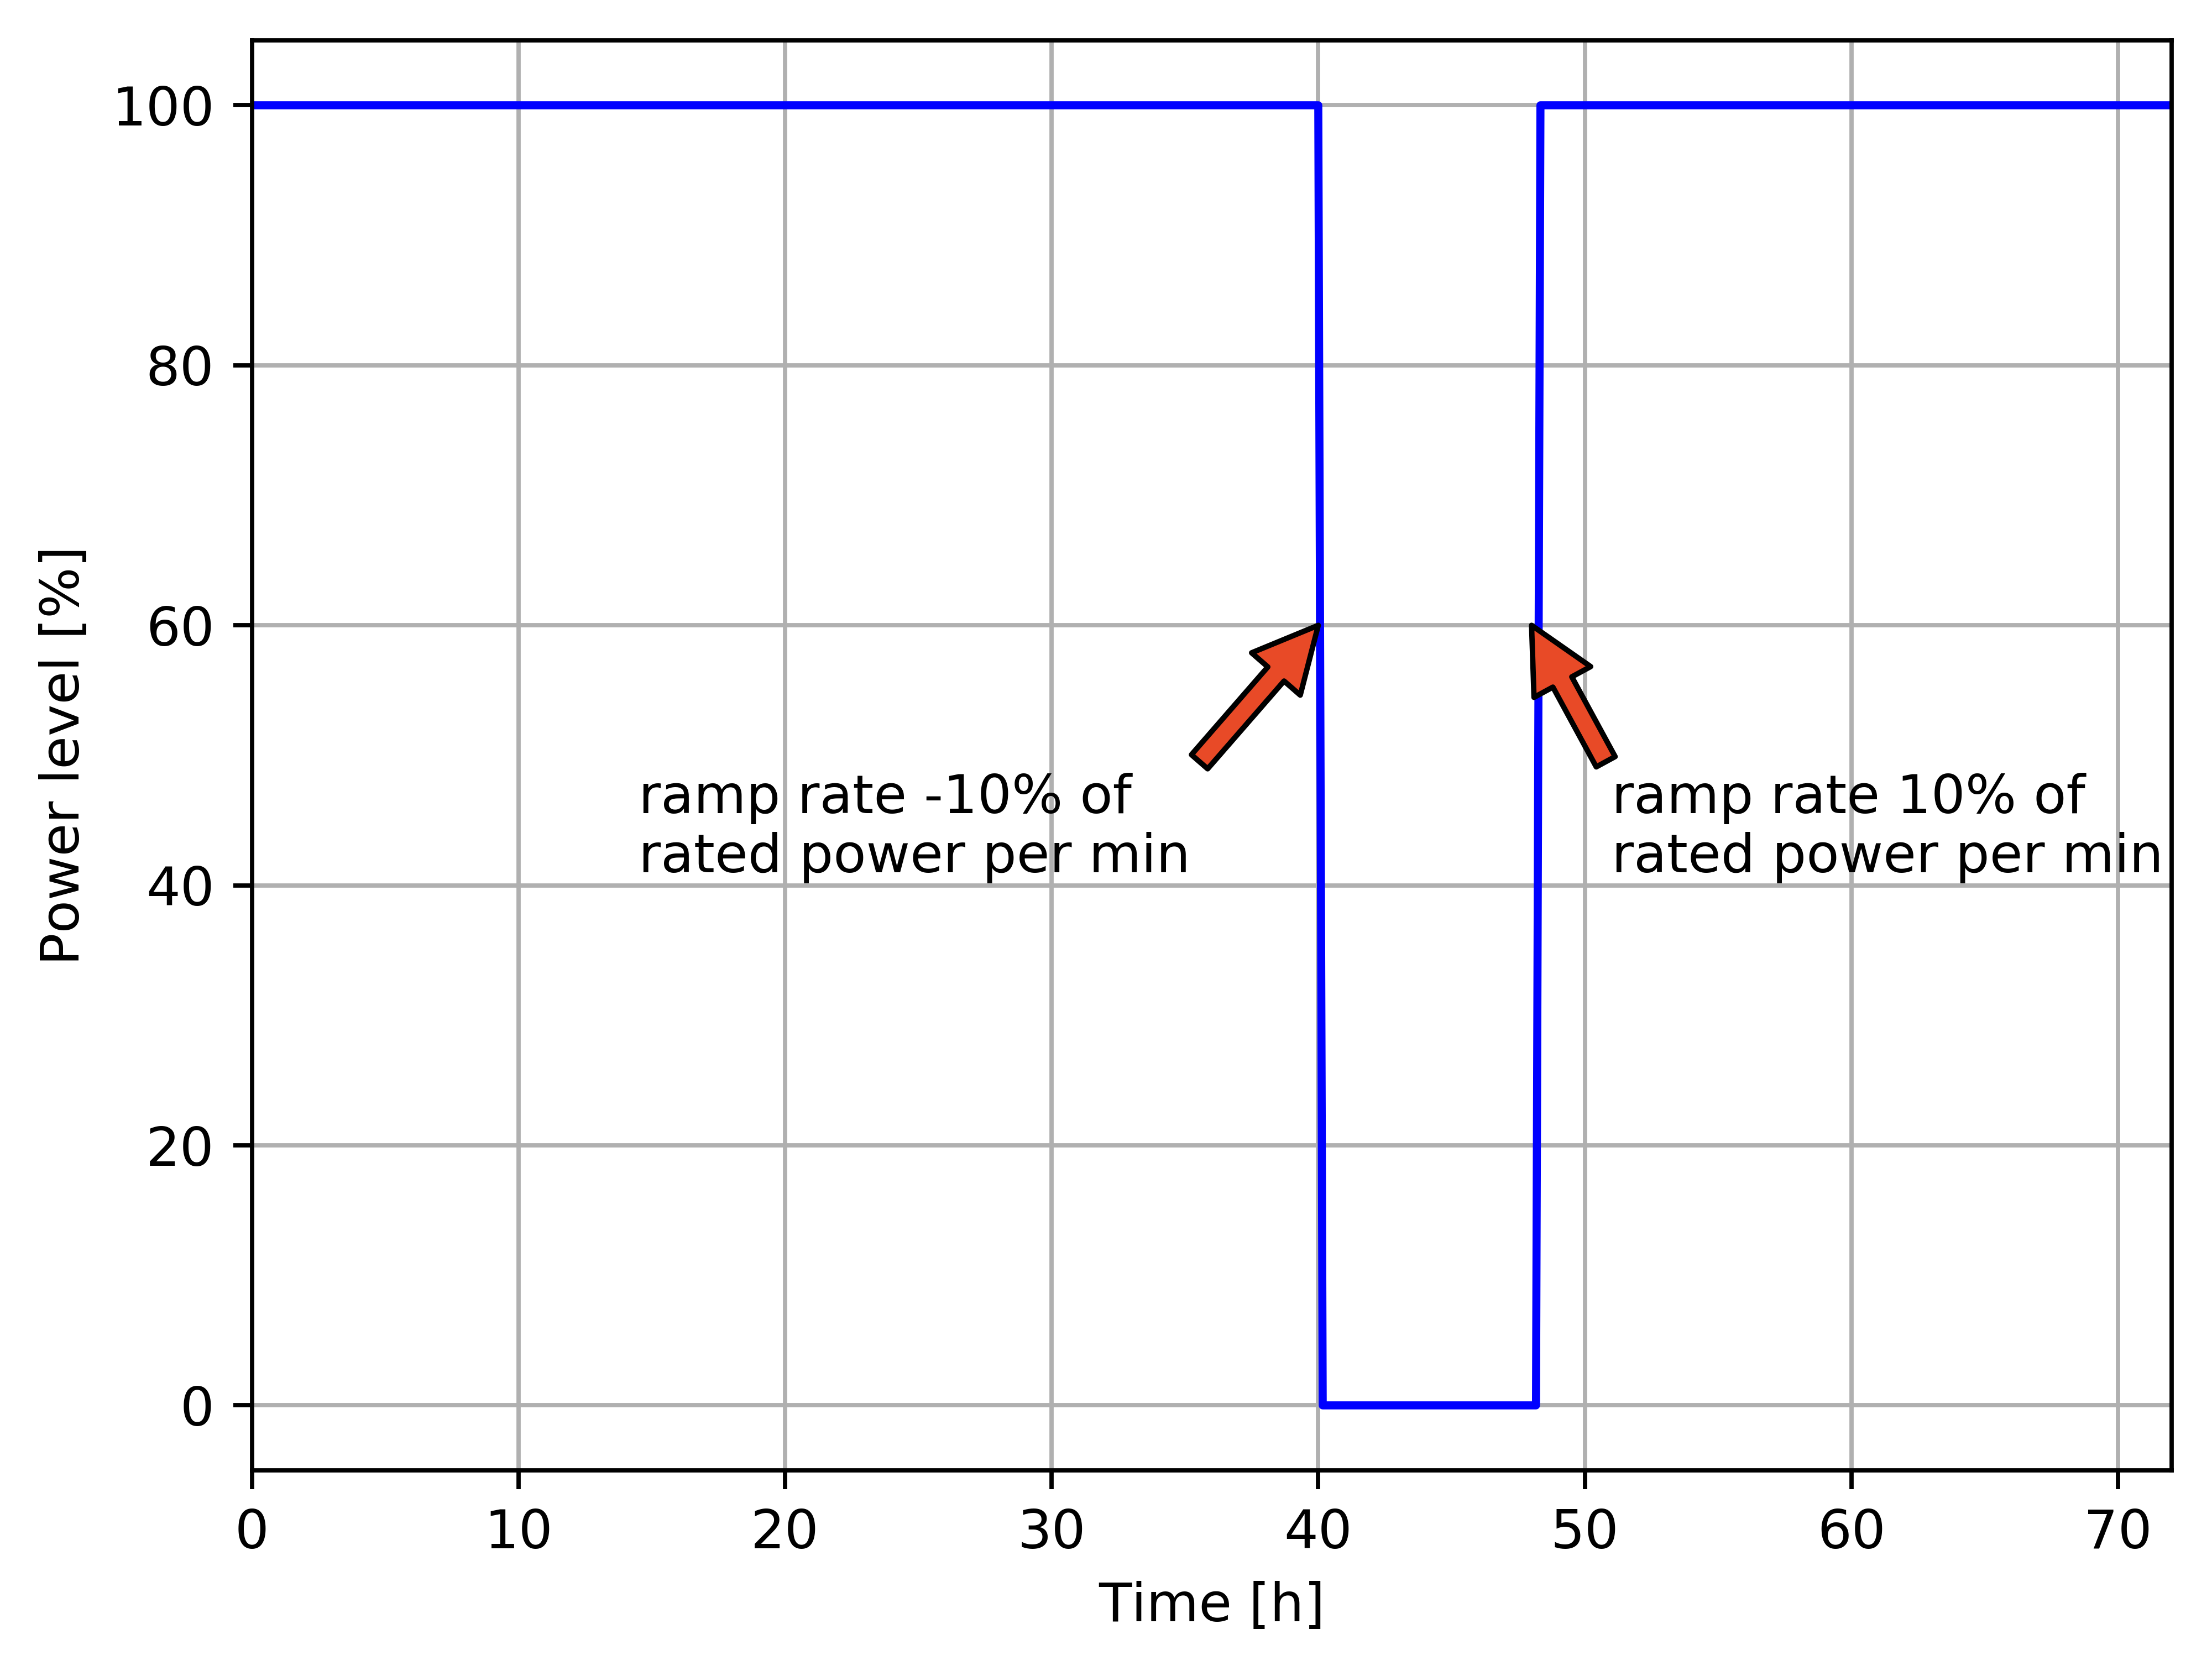
\includegraphics[width=0.8\textwidth]{load_curve.png}
	\caption{Tentative load curve for short-term load-following depletion 
	simulation for the \gls{TAP} reactor using SaltProc v1.0.}
	\label{fig:load}
\end{figure}

The depletion step time for short-term simulation will be varied in a range 
from 1 to 60 min to find a compromise between accuracy and computational cost. 
It is expected that load-following performance will be better at the \gls{BOL} 
because the neutron energy spectrum thermalizes during the reactor operation. 
Thus, the short-term load-following simulation will be repeated for the 
\gls{BOL}, the middle of life, and the \gls{EOL} to assess the \gls{TAP} 
concept performance in a load-following regime during the whole reactor 
lifetime.

Additionally, sensitivity analysis of input parameters in the xenon extraction 
correlation will be conducted to determine the range of key parameters (e.g., 
mass transfer coefficient, helium sparging rate, gas-liquid interfacial area, 
temperature) when load-following is possible for the \gls{TAP} reactor in a 
worst-case power demand scenario. These multiple system configurations  
incorporating user-parametrized components in the fuel salt processing system 
will be collected and published in a \textit{.json}-compatible database for 
use with the SaltProc v1.0 to encourage further research in this area.

\section{Stage 4: Prototype design for the Xe removal system}
As the model becomes capable of incorporating user-parametrized components 
with correlation-based extraction efficiency for the helium sparging 
component, constraints bounding a suitable sparger design will be determined 
and described. These design ranges (i.e., helium sparging rate) obtained from 
the previous Stage. The ultimate objective of the design is to ensure 
load-following operation during most of the operation period when 
minimizing the fuel salt inventory. That is, constrained optimization problem 
must be solved to minimize total fuel salt volume outside of the core. The 
target design parameters for the sparger include: the volume of sparger, 
helium flow rate, salt flow rate, and geometry.

Additionally, nuclear criticality safety analysis will be performed using 
MCNP6 \cite{werner_mcnp6._2018} to confirm that the selected sparger design 
has a subcritical configuration. If the sparger geometry obtained during the 
optimization process is supercritical, the fission gas removal system would 
contain multiple spargers of smaller size connected in parallel. Total fuel 
salt volume and sparger size are expected to be smaller at the \gls{BOL} and 
increase steadily as the neutron energy spectrum becomes softer.

\section{Stage 5: \gls{TAP} Safety Analysis}
The objective of this Stage is to characterize neutronics limits related to 
load following. High-fidelity simulations will achieve this goal with the 
Serpent 2 Monte Carlo code. Specifically, changes in safety parameters 
(Section~\ref{sec:safety-param}) will be evaluated for two time frames:
\begin{enumerate}
	\item Long-time-scale changes in safety parameters should not compromise 
	\gls{TAP} \gls{MSR} safety.
	\item Load-following operation at key moments in the reactor lifetime 
	(e.g., at startup, at the middle of life, at the end of life) must not 
	result in significant changes in safety parameters.
\end{enumerate}
Section~\ref{sec:safety-param-res} showed preliminary calculations of  
temperature coefficients and reactivity control system worth for the \gls{TAP} 
at startup. The next step will develop a axially discretized core geometry in 
Serpent with non-uniform axial density distribution to estimate the axial 
power offset. Afterward, safety parameters will be calculated at the 
\gls{BOL}, the middle of life, and the \gls{EOL} to capture safety parameter  
variation over long time scales. Validation against previous work in a 
collaboration between Transatomic Power and ORNL 
\cite{betzler_assessment_2017, betzler_fuel_2018} will also be 
performed for confidence building. Additionally, analysis for different xenon 
removal efficiencies (i.e., in the range from 0 to 100\%) will be performed to 
capture the effect of $^{135}$Xe concentration on safety.

To analyze the impact of the load-following operation on \gls{TAP} concept 
safety, safety parameter calculations will be repeated for the load-following 
transient. The combination of fuel and moderator temperature coefficients must 
remain strongly negative, and the reactivity worth of control rods must be 
sufficient to shut down the reactor for all times during load-following 
operation. 

\section{Conclusions}
Details of gas removal and fuel salt processing systems in liquid-fueled 
\glspl{MSR} have historically been conceptual rather than concrete. Usually, 
researchers assume ideal rather than realistically constrained poison 
extraction efficiency for reactor performance calculations. This work will 
more realistically model an online molten salt processing system with a focus 
on the gas removal system of the prospective \gls{TAP} \gls{MSR}. SaltProc, a 
Python toolkit was developed as a part of this work. SaltProc couple directly 
with the Serpent 2 Monte Carlo burnup software to capture the evolution of 
fuel salt composition during reactor operation in the context of an online 
fuel processing system.

Modeling and simulation of the online reprocessing system in the \gls{MSR} 
has shown promise in past research. Our work on simulating online fuel  
reprocessing for the thorium-fueled \gls{MSBR} yielded interesting results: 
notable neutron energy spectrum shift and corresponding changes in safety 
parameters during operation. Additional preliminary work also showed promising
results in modeling a simplified fuel processing system for the \gls{TAP} 
\gls{MSR}. These simulations motivate future work in modeling advanced 
liquid-fueled \gls{MSR} plant designs.

To establish a feasible system design for molten salt fuel reprocessing, a 
more advanced model of the \gls{TAP} \gls{MSR} system with adjustable core 
geometry and realistically achievable extraction efficiencies will be 
developed. Extended SaltProc v1.0 will realistically capture the dynamics of 
fuels salt composition changes with higher accuracy. SaltProc v1.0 will also 
be employed to simulate the \gls{TAP} \gls{MSR} behavior in short-term 
transients to determine the feasibility of load following. Additionally, input 
parameters such as flow rates, bubble size, and the void fraction will be 
varied to determine the range of these parameters when the load following is 
possible for the \gls{TAP} concept.

In addition to these simulations, several extensions are suggested to 
advance our preliminary work. First, the feasible design parameters of the 
sparger, critical component of the \gls{TAP} gas removal system, will be 
optimized through sensitivity analysis of geometry and system conditions. To 
guarantee criticality safety, an MCNP6 simulation will be performed to define 
an appropriate sparger geometry. Further effort will focus on safety  
parameter evolution in the \gls{TAP} reactor during lifetime (60 years),  
when the moderator rod configuration discretely changes. Finally, dynamics of 
the safety parameters will be investigated for a short-term case as was 
described in section~\ref{sec:xe-removal-rate}: load following over three days 
with fixed moderator configuration and worst-case scenario of the power level 
change. 

